\documentclass[final,3p,twocolumn]{elsarticle}

\usepackage{amssymb}
\usepackage{mathtools}
\usepackage{tikz}
\usepackage{pgfplots}
\usepackage{algorithm2e}

\biboptions{super, square, sort&compress}

\pgfplotsset{width=\columnwidth, height=0.6\columnwidth, compat=1.8}
\usepgfplotslibrary{groupplots, external}
\tikzexternalize

\journal{MPhil in Scientific Computing}

\begin{document}

\begin{frontmatter}

\title{Multimaterial Simulations using Ghost Fluid Methods}

\author{Knut Sverdrup}

\address{Cavendish Laboratory, Department of Physics, JJ Thomson
  Avenue, Cambridge. CB3 0HE}

\begin{abstract}
    The unsteady, compressible Euler equations for multimaterial flow in one
    dimension have been solved numerically by employing level-set based
    tracking of fronts and two versions of the Ghost Fluid Method. Equations of
    state for stiffened ideal gases are supported, to allow simulations with
    water. An exact Riemann solver is demonstrated, in addition to usage of
    both centered and upwind higher-order time-marching schemes, namely
    MUSCL-Hancock with HLLC and SLIC. Results from several varied test cases
    show that the implementation works in accordance with that presented in
    previous literature. 
\end{abstract}

\end{frontmatter}

\section{Introduction}
\label{sec:introduction}

Leonhard Euler first presented the momentum and continuity equations in 1757
\cite{euler1757principes}, which were completed by the adiabatic condition
presented by Laplace in 1816 \cite{laplace1816vitesse}. The energy balance
equation, which is the last of what is now called the Euler equations,  was not
properly incorporated until the late nineteenth century
\cite{christodoulou2007euler}, and although the much more general Navier-Stokes
equations have been developed \cite{navier1822memoire, stokes1845theories}, the
continued interest for and usefulness of the Euler equations is undisputable.
They provide a robust framework for analyzing ideal fluids when viscuous
effects are negligible, but cannot generally be solved analytically.
Applications of the Euler equations include aerodynamics
\cite{drela1985twodimensional, anderson1986comparison, guruswamy1990unsteady},
atmospheric modelling and weather forecasts \cite{laprise1992euler,
skamarock2008time}, astrophysics \cite{trac2003primer} and detonations and
explosives \cite{nikiforakis1996numerical, williams1996detailed,
saurel2001multiphase}, to name a few.  Accordingly, precise and efficient
methods for solving these non-linear, hyperbolic partial differential equations
on arbitrary domains has been, and still is, a major field in modern
computational fluid dynamics. 

The Euler equations govern adiabatic and inviscid flow of a fluid. In the
Froude limit (no external body forces) in one dimension, with density $\rho$,
velocity $u$, total energy $E$ and pressure $p$, they are given by 

\begin{equation}
    \partial_t {\bf U} + \partial_x {\bf F(U)} = 0\,,
    \label{eq:euler}
\end{equation}
%
where the vector of conserved quantities ${\bf U}$ and their fluxes ${\bf F(U)}$ are given by

\begin{equation*}
    {\bf U} = 
    \begin{bmatrix} 
        \rho \\ 
        \rho u \\ 
        E 
    \end{bmatrix}
    \,,\quad
    {\bf F} = 
    \begin{bmatrix}
        \rho u \\ 
        \rho u^2 + p \\
        u(E+p) 
    \end{bmatrix}
    \,.
\end{equation*}
%
It is sometimes convenient to work in terms of the primitive variables ${\bf W} =
\begin{pmatrix} \rho, & u, & p \end{pmatrix}^T$. The total energy is the sum of
the kinetic and potential energy of the system, i.e.~ 

\begin{equation}
    E = \frac{1}{2} \rho u^2 + \rho e \,,
    \label{eq:energy}
\end{equation}
%
where $e$ is the internal energy, related to the other variables through the
equation of state. For an ideal gas, the equation of state is 

\begin{equation}
     e = \frac{p}{(\gamma-1)\rho} \,,
     \label{eq:EoS}
 \end{equation}
%
where $\gamma$ denotes the ratio of specific heats for the gas. Several other
fluids can be approximated by a so-called stiffened ideal gas equation of
state, 

\begin{equation}
    e = \frac{p+\gamma p_{\infty}}{(\gamma-1)\rho} \,.
    \label{eq:stiffEoS}
\end{equation}
%
Here, a material-dependent stiffening parameter $p_{\infty}$ has been
introduced. Note that Eq.\ \eqref{eq:stiffEoS} reduces to Eq. \eqref{eq:EoS} for
materials with $p_{\infty}=0$.

Many important milestones have led us to the current state of the art of
solving the Euler equations numerically. Riemann identified and worked on the
initial value problem for Eq.\ \eqref{eq:euler} with discontinuous initial
conditions as early as 1860 \cite{riemann1860fortpflanzung}, but the first
exact solution did not arrive until Godunov proposed an iterative scheme a
century later \cite{godunov1959difference}. Today, efficient approximate
solvers such as HLLC (Harten-Lax-van Leer-Contact) \cite{toro1994restoration}
and Rotated-hybrid Riemann solvers \cite{nishikawa2008very} are readily
available. The development of numerical analysis methods for partial
differential equations got its first proper boost after the famous paper by
Courant, Friedrichs and Lewis \cite{courant1928partiellen}, but local Riemann
problems \cite{godunov1959difference}, conservative methods
\cite{lax1960systems} and finite volume formulations \cite{leveque2002finite}
were necessary before the first proper, three-dimensional simulations of the
Euler equations could be performed in the 1980s \cite{jameson1981numerical}.
After the Monotonic Upstream-centered Scheme for Conservation Laws (MUSCL)
\cite{van1979towards} was introduced by van Leer as the first higher-order
Total Variation Diminishing (TVD) scheme in 1979, several others have been
developed, notably Toro's Weighted Average Flux (WAF) \cite{toro1989weighted} and
Flux/Slope LImiter Centred (SLIC/FLIC) \cite{toro2000centred} schemes. 

Considerations of multimaterial interactions and flow are among the more recent
(less than twenty year old) developments within numerical solutions for the
Euler equations. It is the goal of this report to demonstrate some techniques
available for multimaterial simulations of the Euler equations in one
dimension. Different fluids are characterized by their material properties,
such as $\gamma$, and thus special care must be taken in the treatment of
boundaries separating different fluids. 

Firstly, the location of the boundary must be tracked as time evolves. The most
common way of doing this is by the use of level set methods, as proposed by
Osher and Sethian \cite{osher1988fronts}. The level set function for a region
is initiated such that it is negative inside the region, positive outside it
and zero on the boundary. By taking into consideration the convection of the
fluids under consideration, the level set function is then evolved so that its
zeros move with the domain boundary. Osher and Fedkiw \cite{osher2001level}
provide an excellent overview of level set methods and their applications. 

Secondly, the interaction between different fluids across the material
interfaces must be modelled accurately. In order to do so, Fedkiw \emph{ et
al.\ } developed the Original Ghost Fluid Method (OGFM)
\cite{fedkiw1999nonoscillatory}. In ghost fluid methods, each material has
ghost cells on the side of the boundary where the other material exists. In the
OGFM, the pressures and velocities at these ghost cells are similar to that of
the other material, and the densities are calculated by enforcing constant
entropy across the interface. This worked well for cases except when there were
strong shock waves, since the entropy condition does not apply. As a response,
the Modified Ghost Fluid Method (MGFM) was developed \cite{liu2003ghost,
sambasivan2009ghost}. It is based on the realization that Riemann problems do
not in general require the states on each side of the discontinuity to
correspond to the same material. The cells in the ghost fluid are therefore
updated by solving a local Riemann problem. A further development is the real
Ghost Fluid Method (rGFM) \cite{wang2006real}, in which a more accurate
interfacial boundary condition is applied. The implementation of the rGFM is
outside the scope of this report. 

The numerical methods which have been employed are explained in section
\ref{sec:numerical}, before several test cases and their results are discussed
in section \ref{sec:results}. Section \ref{sec:conclusion} concludes the
report.

\section{Numerical methods}
\label{sec:numerical}

\subsection{Riemann solvers}
\label{subsec:riemann}

Given a conservation equation and two sets of piecewise constant states
separated by a single discontinuity, the initial value problem of evolving this
system in time is called a Riemann problem. It is very useful in the study of
the Euler equations for two reasons. Firstly, it allows for exact (up to an
arbitrary accuracy) solutions for systems obeying Eq.\  \eqref{eq:euler} which
have a single contact discontinuity. The other benefit of Riemann solvers is
that the discretization of space which is inevitable in computational schemes
for solving differential equations, allows for precise solvers of conservation
equations based on the solutions of many local Riemann problems. 

For the Euler equations and initial conditions 

\begin{equation*}
    {\bf W}(x,t=0) = 
    \begin{cases}
        {\bf W}_L, \,&x \leq 0 \\ 
        {\bf W}_R, \,&x > 0 \\ 
    \end{cases} \,,
\end{equation*}
%
typical states the system can have are shown in Figure \ref{fig:riemann}, in
addition to characteristics for waves propagating in space-time. There are two
types of resultant waves that propagate through space, in addition to the
contact wave (dashed). The first is a shock wave, depicted as a thick line on
the left, while the second is a rarefaction wave, shown as several gradually
decaying lines on the right. Four different combinations of shock and
rarefaction waves can occur on the left and right sides of the contact
discontinuity, and the result is only dependent on ${\bf W}(x,0)$. 

\begin{figure}[htb]
    \centering
    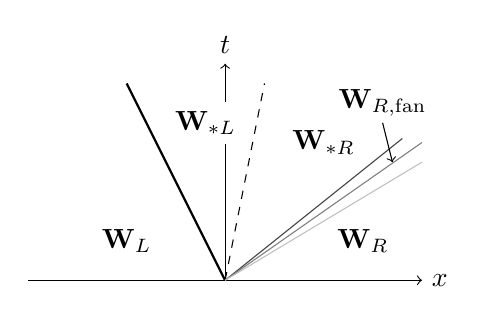
\begin{tikzpicture}[scale=2.5]
        \coordinate (origin) at (0,0);
        \coordinate (left) at (-1,0);
        \coordinate (right) at (1,0);
        \coordinate (top) at (0,1.1);
        \draw[->] (left) -- (right) node[right]{$x$};
        \draw[->] (origin) -- (top) node[above]{$t$};
        \draw[thick] (origin) -- (-0.5,1) {};
        \draw[dashed] (origin) -- (0.2,1) {};
        \draw[black!75] (origin) -- (0.9,0.72) {};
        \draw[black!50] (origin) -- (1,0.7) {};
        \draw[black!25] (origin) -- (1,0.6) {};
        \node () at (-0.5,0.2) {${\bf W}_L$};
        \node[fill=white] () at (-0.1,0.8) {${\bf W}_{*L}$};
        \node () at (0.5,0.7) {${\bf W}_{*R}$};
        \node () at (0.8,0.9) {${\bf W}_{R,{\rm fan}}$};
        \draw[<-] (0.85,0.6) -- (0.8,0.8) {};
        \node () at (0.7,0.2) {${\bf W}_R$};
    \end{tikzpicture}
    \caption{Possible wave configurations for the Riemann problem for Euler's
    equations in one dimension.}
    \label{fig:riemann}
\end{figure}

As seen from Figure \ref{fig:riemann}, there are (up to) four unknown states
for the Riemann problem: the left and right star states ${\bf W}_{*K}$ located
between the left and right waves, and additionally the states inside
rarefaction waves ${\bf W}_{K, {\rm fan}}$. Note that the density in the $K$
star state depends on whether the corresponding wave is of shock of rarefaction
type. One must therefore be able to compute all these states, and also
determine which of them is the correct one based on the speeds of the waves. 

\subsubsection{Exact solver}
\label{subsubsec:exact}

The exact solver, as first introduced by Godunov \cite{godunov1959difference},
has been implemented following Chapter 4 of Toro's comprehensive overview of
Riemann solvers and their uses \cite{toro2013riemann}, but extended to take
into consideration that different (stiffened) ideal gases may be present on
each side of the discontinuity. 

It can be proven that the pressure in the star states $p_{*}$ is given by
the root of the nonlinear function

\begin{equation}
    f(p) = f_L(p)+f_R(p)- (u_L-u_R) \,.
    \label{eq:pressureEquation}
\end{equation}
%
Here,  

\begin{equation*}
    f_K(p) = 
    \begin{cases}
        \frac{2a_K}{\gamma_K-1} \left[ \left(
            \frac{p+p_{\infty,K}}{p_K+p_{\infty,K}}
        \right)^{\frac{\gamma_K-1}{2\gamma_K}}-1\right], &p\leq p_K \\
        (p-p_K)\left( \frac{A_K}{B_K+p} \right)^{\frac{1}{2}}, &p>p_K
    \end{cases} \,,
\end{equation*}
%
where $a_K = \sqrt{\frac{\gamma(p_K+p_{\infty,K})}{\rho_K}}$ is the speed of
sound and 

\begin{equation*}
    A_K = \frac{2}{(\gamma_K+1)\rho_K} \,,\,
    B_K = \frac{(\gamma_K-1)p_K+2\gamma_K p_{\infty, K}}{\gamma_K+1} \,.
\end{equation*}
% 
In the exact solver, the pressure in the star region is found by applying an
iterative scheme to Eq.~ \eqref{eq:pressureEquation}. Due to the nature of
$f(p)$, it is well-suited for iterative schemes, but
it is important to ensure that the pressure stays positive. For this project,
Newton-Raphson iterations were implemented, taking the initial guess as
$\frac{1}{2}(p_L+p_R)$. After finding $p_*$, the velocity in the star region is computed as

\begin{equation}
    u_{*} = \frac{u_L+u_R-[f_L(p_*)-f_R(p_*)]}{2} \,.
    \label{eq:ustar}
\end{equation}

When the pressure and velocity in the star region have been computed, one can
calculate the wave speeds (one per shock wave, two per rarefaction wave and one
for the contact discontinuity) and use this to sample the state at a given
point $S = x/t$ in space-time. Pseudocode for this procedure is given in
Algorithm \ref{alg:sample}. Formulas for wave speeds and densities in different
states have been left out for brevity, but they in general depend on the
initial conditions (including material properties).

\begin{algorithm}[htb]
    \KwData{$S$, ${\bf W}_L$, ${\bf W}_R$, $p_{*}$, $u_{*}$, material
properties}
    \KwResult{${\bf W}(S)$}
    \eIf{$S \leq$ \rm speed of contact discontinuity}
    {
        \eIf{\rm left wave is rarefaction}
        {
            \eIf{$S \leq $ \rm speed of rarefaction head}
            {
                return ${\bf W}_L$\;
            }
            {
                \eIf{$S >$ \rm speed of rarefaction tail}
                {
                    return ${\bf W}_{*L, {\rm fan}}$\;
                }
                {
                    return ${\bf W}_{L, {\rm fan}}$\;
                }
            }
        }
        {
            \eIf{$S \leq $ \rm speed of shock wave}
            {
                return ${\bf W}_L$\;
            }
            {
                return ${\bf W}_{*L}$\;
            }
        }
    }
    {
        perform similar analysis for sampling point on right side of contact
        discontinuity; 
    }
    \caption{Sample exact solution of Riemann problem given pressure and
    velocity in star states.}
    \label{alg:sample}
\end{algorithm}

\subsubsection{HLLC}
\label{subsubsec:hllc}

By far the most computationally expensive part of the exact solver is the
iterative root finding procedure for finding $p_*$. Since most modern schemes
require the solutions of local Riemann problems between all points in the
computational domain, high gains in terms of computational efficiency can be
achieved by employing exact solvers instead. One such solver is the HLLC solver
\cite{toro1994restoration}, which has been implemented for this project. 

When compared to the exact solver, the main simplifications in HLLC are that
the pressure in the star region is approximated instead of found by iterative
schemes; that states inside rarefactions are not taken into consideration, and 
that wave speeds are estimations, either direct or pressure-based. In this
contribution, the pressure is estimated as 

\begin{equation}
    p_* \approx \frac{1}{2}(p_L+p_R) 
    +\frac{1}{8}(u_L-u_R)(\rho_L+\rho_R)(a_L+a_R) \,,
    \label{eq:pressureHLLC}
\end{equation}
%
and set equal to zero if the approximation is negative. Based on the
approximation for $p_*$, the wave speeds $S_K$ of the left and right travelling
waves are computed, with the type of wave taken into consideration. The speed
of the contact discontinuity is then approximated as

\begin{equation}
    S_* \approx \frac{\rho_L u_L(S_L-u_L)-\rho_R
    u_R(S_R-u_R)-(p_L-p_R)}{\rho_L(S_L-u_L)-\rho_R(S_R-u_R)} \,.
    \label{eq:speedHLLC}
\end{equation}

There are four possible states, separated by the three (approximated) wave
speeds.  Contrary to the exact solver, where the output is the state ${\bf
W}(S)$, the HLLC solver outputs a flux ${\bf F}^{\rm HLLC}({\bf W}_L, {\bf
W}_R)$ based on the state corresponding to $S=0$. This is because the flux at
the intermediate point between cells is the quantity employed in the update
formula as introduced in Subsection \ref{subsec:eulerschemes}. For an overview
of the approximate states and the flux calculation employed in the HLLC solver,
see Chapter 9 of Toro's book \cite{toro2013riemann}. 

\subsection{Schemes for the Euler equations}
\label{subsec:eulerschemes}

The Euler equations as given in Eq.\ \eqref{eq:euler} are said to be a system
of conservation equations in differential form. In integral form, on a spatial
domain $[x_L, x_R]$, the same system of equations can be written

\begin{align}
    \nonumber
    \int_{x_L}^{x_R} {\bf U}(x,t_2) {\rm d}x = 
    \int_{x_L}^{x_R} &{\bf U}(x,t_1) {\rm d}x \\ 
    -\int_{t_1}^{t_2} {\bf F}({\bf U}(x_R,t)) {\rm d}t 
    &+ \int_{t_1}^{t_2} {\bf F}({\bf U}(x_L,t)) {\rm d}t \,.
    \label{eq:eulerIntegral}
\end{align}

From Eq. \eqref{eq:eulerIntegral}, it is straightforward to discretize the
Euler equations to produce a conservative time-marching scheme through the
Finite Volume Method (FVM). Let the spatial domain $x \in [0,1]$ be divided
into $N$ equal cells of width $\Delta x = 1/N$.  We denote by $x_i$ the center
of the $i$-th cell, \emph{i.e.~} $x_i = (i+1/2)\Delta x$. 
%
Temporal discretization is done with variable time step $\Delta t^n$, so that
$t^n = \sum_{i=1}^n \Delta t^i$. 

We write the discrete
approximation of ${\bf U}(x_i, t^n)$ as ${\bf U}_i^n$, and let it be the
weighted average of ${\bf U}(x,t^n)$ in the cell with boundaries at
$x_{i-1/2}$ and $x_{i+1/2}$: 

\begin{equation}
    {\bf U}_i^n \approx \frac{1}{\Delta x} \int_{x_{i-1/2}}^{x_{i+1/2}} {\bf
    U}(x,t^n) {\rm d}x 
    \label{eq:Udiscrete}
\end{equation}
%
Similarly, the fluxes at each interface are approximated as 

\begin{equation}
    {\bf F}_{i+1/2}^n \approx \frac{1}{\Delta t^n} 
    \int_{t_{n}}^{t_{n+1}} {\bf F}({\bf U}(x_{i+1/2},t)) {\rm d}t \,. 
    \label{eq:Fdiscrete}
\end{equation}
%
By applying Eq. \eqref{eq:eulerIntegral} on each cell $[x_{i-1/2},x_{i+1/2}]$,
and by inserting the discrete approximations in Eqns. \eqref{eq:Udiscrete} and
\eqref{eq:Fdiscrete}, a conservative, time-marching scheme for evolving the
Euler equations in time is 

\begin{equation}
    {\bf U}_i^{n+1} = {\bf U}_i^n - \frac{\Delta t^n}{\Delta x} \left(
    {\bf F}_{i+1/2} - {\bf F}_{i-1/2} \right) \,. 
    \label{eq:conservativeScheme}
\end{equation}
%
The Courant-Friedrichs-Lewis condition for convergence demands that 

\begin{equation}
    \label{eq:timeStep}
    \Delta t^n \leq \frac{\Delta x}{S_{\rm max}^n} \,,
\end{equation}
%
so we let $\Delta t^n = C_{\rm CFL} \Delta x / S_{\rm max}^n$, where $0 \leq
C_{\rm CFL} \leq 1$. In our implementation, we use $C_{\rm CFL}=0.9$.
Transmissive boundary conditions are implemented on both boundaries, so that

\begin{equation}
    \label{eq:BCs} 
    {\bf W}_{-i}^{n+1} = {\bf W}_{-(i-1)}^{n} \,, \quad
    {\bf W}_{N+i}^{n+1} = {\bf W}_{N+(i-1)}^{n} \,, \quad 
\end{equation}
%
for $i=1, \dots, N_{GC}$ where the number of ghost cells $N_{GC}$ equals the
order of the scheme employed. 

All the most common schemes used for solving conservation laws are of the same
form as Eq. \eqref{eq:conservativeScheme}, and the difference between them is
in the evaluation of the fluxes ${\bf F}_{i\pm 1/2}$. For this project, we have
implemented so-called total variation diminishing (TVD) high resolution methods
for this purpose. High resolution methods are accurate to at least second
order; they avoid spurious oscillations in the solution, capture
discontinuities and shock waves well and satisfy a discrete form of the entropy
condition. There are two main classes of higher-order flux evaluation schemes;
the upwind schemes are based on the solution of local Riemann problems, while
the centered schemes are extensions of the First ORder CEntered (FORCE) flux: 

\begin{align} 
    \nonumber 
    {\bf F}^{\rm FORCE}({\bf U}_L,{\bf U}_R) = \frac{1}{2}
    &\left[ {\bf F}_0 + \frac{1}{2} ({\bf F}_L + {\bf F}_{R})
    \right] \\
    \label{eq:FORCE} 
    &- \frac{1}{4} \frac{\Delta x}{\Delta t^n} ({\bf U}_{R} - {\bf
    U}_L) \,.  
\end{align}
%
Here, ${\bf F}_K = {\bf F}({\bf U}_K)$ and 

\begin{equation}
    \label{eq:richtmyer}
    {\bf U}_0 = \frac{1}{2}({\bf U}_L+{\bf U}_R) -
    \frac{1}{2} \frac{\Delta t}{\Delta x}({\bf F}_R - {\bf F}_L) \,.
\end{equation}
%
In general, upwind schemes offer higher accuracy than centered once, but they
are computationally more demanding and difficult to implement. 

The MUSCL-Hancock \cite{van1979towards} and SLIC \cite{toro2000centred}
schemes, as mentioned in the Introduction, exemplify upwind and centred
schemes, respectively. They are similar in many regards, and both consist of
three main steps. 

First, the data cell averages ${\bf U}_i^n$ are replaced
locally by linear functions so that at the left and right cell interfaces, the
boundary extrapolated values are 

\begin{equation}
    \label{eq:BEV}
    {\bf U}_i^L = {\bf U}_i^n-\frac{1}{2}\Delta_i \,,\quad 
    {\bf U}_i^R = {\bf U}_i^n+\frac{1}{2}\Delta_i \,.
\end{equation}
%
Here, the slope vector $\Delta_i$ has been introduced, which in our case is
chosen such that the schemes are TVD. For the MUSCL-Hancock scheme, we have
implemented limited slopes \cite{anderson1986comparison}, while SLIC uses slope
limiters \cite{toro2000centred}. 

After calculating the boundary extrapolated values for each cell, these are
advanced to time $t^n+\Delta t^n$ to obtain

\begin{equation}
    \label{eq:evolution}
    {\bf \bar{U}}_i^{L,R} = {\bf U}_i^{L,R} - \frac{1}{2} \frac{\Delta
    t}{\Delta x} \left[ {\bf F}({\bf U}_i^R)-{\bf F}({\bf U}_i^L) \right] \,.
\end{equation}

The third and final step is the actual evaluation of the intercell flux ${\bf
F}_{i+1/2}$ based on the partially evolved boundary extrapolated values. For
MUSCL-Hancock, this is done by using the HLLC solver to solve the local Riemann
problem across each cell interface, \emph{i.e.~} 

\begin{equation}
    \label{eq:MUSCL}
    {\bf F}_{i+1/2}^{\rm MUSCL} = {\bf F}^{\rm HLLC}({\bf
    \bar{W}}_i^R, {\bf \bar{W}}_{i+1}^L) \,.
\end{equation}
%
For SLIC, however, the intercell flux is directly evaluated as the FORCE flux with 

\begin{equation}
    \label{eq:SLIC}
    {\bf F}_{i+1/2}^{\rm SLIC} = {\bf F}^{\rm FORCE}({\bf
    \bar{U}}_i^R, {\bf \bar{U}}_{i+1}^L) \,.
\end{equation}
\subsection{Level-set method}
\label{subsec:levelset}

In order to represent the interfaces between materials, we employ a level-set
function $\phi(x)$ whose sign is a boolean indicator of the material present. The
interfaces between materials are thus located at the points where $\phi=0$.
Figure \ref{fig:levelSet} shows the simple case of a single material interface
separating materials A and B; several interfaces have been incoorporated by
letting $\phi$ be piecewise linear throughout the domain in a zig-zag
pattern. 

\begin{figure}[htb]
    \centering
    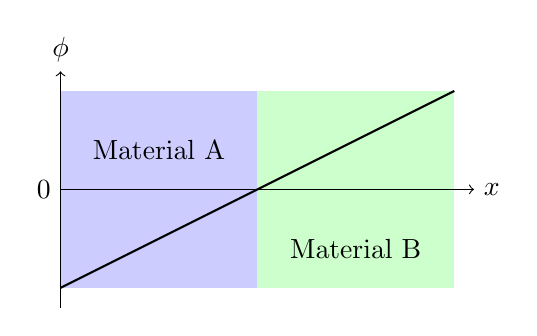
\begin{tikzpicture}[scale=2.5]
        \coordinate (origin) at (0,0) node[left]{0};
        \coordinate (mid) at (1,0);
        \coordinate (xright) at (2.1,0);
        \coordinate (bottom) at (0,-0.6);
        \coordinate (top) at (0,0.6);
        \coordinate (yleft) at (0,-0.5);
        \coordinate (yright) at (2,0.5);
        \coordinate (dashtop) at (1,0.5);
        \coordinate (dashbottom) at (1,-0.5);

        \fill[blue!20!white] (yleft) rectangle (dashtop);
        \fill[green!20!white] (dashbottom) rectangle (yright);

        \draw[->] (origin) -- (xright) node[right]{$x$};
        \draw[->] (bottom) -- (top) node[above]{$\phi$};
        \draw[thick] (yleft) -- (yright) {};

        \node[fill=blue!20!white] () at (0.5,0.2) {Material A};
        \node[fill=green!20!white] () at (1.5,-0.3) {Material B};
    \end{tikzpicture}
    \caption{Simple example of level-set function for one material interface.
    In the left region, where $\phi(x)<0$, material A is present,
    while material B is present in the right region. }
    \label{fig:levelSet}
\end{figure}

Initializing the level-set function is trivial, but it is a good idea to make
sure that the zeros end up between cell centers, so that each grid point has
well-defined material properties. In order to capture the evolution of the
system, the level-set function itself must be advanced in time for each time
step. Since $\phi$ is a consequence of the state of the fluid rather than a
property, it is not coupled to the other variables in the system.  Thus it is
governed by the advection equation 

\begin{equation}
    \label{eq:phi}
    \partial_t \phi + u\partial_x \phi = 0 \,,
\end{equation}
%
Due to frequent discontinuities in density at material interfaces, conservative
schemes lead to smearing of the locations of the zeros. Since the only
interesting information contained in $\phi$ are these locations,
non-conservative methods can be safely implemented as long as $\phi$ remains
smooth and not too sharp. In our implementation, we have implemented the
first-order upwind scheme 

\begin{equation}
    \label{eq:advanceLevelSet}
    \phi_i^{n+1} = \begin{cases}
        \phi_i^n-u_i^n \frac{\Delta t^n}{\Delta x}(\phi_i^n-\phi_{i-1}^n)
        \,,\quad u_i^n > 0 \\
        \phi_i^n-u_i^n \frac{\Delta t^n}{\Delta x}(\phi_{i+1}^n-\phi_i^n) 
        \,,\quad u_i^n \leq 0
    \end{cases} \,.
\end{equation}
%
Note that $u_i^n$ is the velocity of material A at $x_i$ if $\phi_i^n < 0$, and
the velocity of material B otherwise.  In order to avoid the level set function
becoming too sharp, we reinitialize it after every update by demanding
$|\phi_{i+1}^n-\phi_i^n|=\Delta x$. In this procedure, we also make sure that
the zeros of $\phi$ lie between grid points. 

\subsection{Ghost fluid methods}
\label{subsec:ghostfluid}

Multimaterial simulations require one final consideration in addition to
interface tracking; namely which boundary conditions to enforce across these
interfaces. These dynamic boundary conditions should be thermodynamically
consistent in order to capture the physical interactions between materials. In
the computational implementation, the Euler equations are solved on a separate
domain for each material, where that material is present in all cells. For the
regions where $\phi(x) < 0$, fluid A is present in domain A, while \emph{ghost
fluid} B is present in domain B. The opposite is true when $\phi(x) > 0$. The
only interesting cells in the ghost fluids are the $N_{GC}$ points located
immediately adjacent to a material interface, since these affect the solution
in the actual fluid. It is the goal of ghost fluid methods to update these
ghost cells in a thermodynamically consistent manner. 

\subsubsection{Original ghost fluid method}
\label{subsubsec:ogfm}

The first successful attempt at implementing a ghost fluid method was performed by
Fedkiw et al.~ in 1998 \cite{fedkiw1999nonoscillatory}. In this approach, which
we refer to as OGFM, the entropy $S$ is held constant across the ghost fluid
interface, in order to give conditions for thermodynamic consistensy. The
assumption of constant entropy is not entirely true in the case of shocks, so
one does not expect excellent capturing of large shock waves. The pressure and
velocity in the ghost cells are set equal to the pressure and velocity in the
same cells of the other material domain. It is the density which is
extrapolated by enforcing constant entropy. To derive how, we note that the
entropy of an ideal gas is given by 

\begin{equation}
    \label{eq:entropy}
    S = c_V \ln \left( \frac{p}{\rho^{\gamma}} \right) + {\rm const} \,,
\end{equation}
%
so if two cells $i$ and $j$ have the same entropy and contain the same
material, they must satisfy 

\begin{equation}
    \label{eq:constEntropy}
    \rho_i = \left( \frac{p_i}{p_j} \right)^{1/\gamma} \rho_j \,.
\end{equation}
%
In order to avoid ``overheating'' across the material boundary, an isobaric fix
has been implemented for OGFM by enforcing constant entropy from the neighbour
of the boundary cell to the boundary as well as from the boundary and into
the ghost fluid. A schematic illustration, including the isobaric fix, is given
in Figure \ref{fig:OGFM}. 

\begin{figure}[htb]
    \centering
    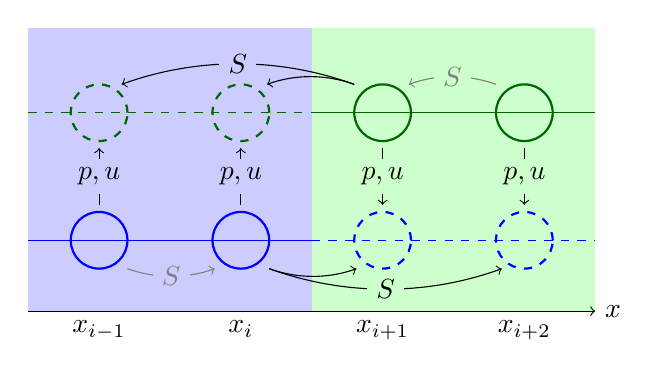
\begin{tikzpicture}[scale=1.8]
        \coordinate (origin) at (0,0);
        \coordinate (x0) at (-1.5,0);
        \coordinate (x1) at (-0.5,0);
        \coordinate (x2) at (0.5,0);
        \coordinate (x3) at (1.5,0);
        \coordinate (y0) at (-1.5,0.5);
        \coordinate (y1) at (-0.5,0.5);
        \coordinate (y2) at (0.5,0.5);
        \coordinate (y3) at (1.5,0.5);
        \coordinate (z0) at (-1.5,1.4);
        \coordinate (z1) at (-0.5,1.4);
        \coordinate (z2) at (0.5,1.4);
        \coordinate (z3) at (1.5,1.4);
        \coordinate (bottomLeft) at (-2,0);
        \coordinate (topMid) at (0,2);
        \coordinate (bottomRight) at (2,0);
        \coordinate (topRight) at (2,2);

        \fill[blue!20!white] (bottomLeft) rectangle (topMid);
        \fill[green!20!white] (origin) rectangle (topRight);

        \draw[thick,blue] (y0) circle (0.2);
        \draw[thick,blue] (y1) circle (0.2);
        \draw[thick,blue,dashed] (y2) circle (0.2);
        \draw[thick,blue,dashed] (y3) circle (0.2);
        \draw[thick,green!40!black,dashed] (z0) circle (0.2);
        \draw[thick,green!40!black,dashed] (z1) circle (0.2);
        \draw[thick,green!40!black] (z2) circle (0.2);
        \draw[thick,green!40!black] (z3) circle (0.2);

        \draw[->] ($(y0)+(0,0.25)$)--($(z0)-(0,0.25)$) 
        node[fill=blue!20!white,midway]{$p,u$};
        \draw[->] ($(y1)+(0,0.25)$)--($(z1)-(0,0.25)$) 
        node[fill=blue!20!white,midway]{$p,u$};
        \draw[<-] ($(y2)+(0,0.25)$)--($(z2)-(0,0.25)$) 
        node[fill=green!20!white,midway]{$p,u$};
        \draw[<-] ($(y3)+(0,0.25)$)--($(z3)-(0,0.25)$) 
        node[fill=green!20!white,midway]{$p,u$};

        \draw[->] ($(y1)+(0.2,-0.2)$) arc (250:290:0.9);
        \draw[->] ($(y1)+(0.2,-0.2)$) arc (250:290:2.4)
        node[fill=green!20!white,midway]{$S$};
        \draw[black!50!white,->] ($(y0)+(0.2,-0.2)$) arc (250:290:0.9)
        node[black!50!white,fill=blue!20!white,midway]{$S$};

        \draw[->] ($(z2)-(0.2,-0.2)$) arc (70:110:0.9);
        \draw[->] ($(z2)-(0.2,-0.2)$) arc (70:110:2.4)
        node[fill=blue!20!white,midway]{$S$};
        \draw[black!50!white,->] ($(z3)-(0.2,-0.2)$) arc (70:110:0.9)
        node[black!50!white,fill=green!20!white,midway]{$S$};

        \draw[->] (bottomLeft) -- (bottomRight) node[right]{$x$};
        \draw[blue] (-2,0.5)--(0,0.5) {};
        \draw[blue,dashed] (0,0.5)--(2,0.5) {};
        \draw[green!40!black,dashed] (-2,1.4)--(0,1.4) {};
        \draw[green!40!black] (0,1.4)--(2,1.4) {};
        \node[below] () at (x0) {$x_{i-1}$};
        \node[below] () at (x1) {$x_{i}$};
        \node[below] () at (x2) {$x_{i+1}$};
        \node[below] () at (x3) {$x_{i+2}$};
    \end{tikzpicture}
    \caption{Updating of cells in ghost fluids as implemented in OGFM. The
    pressure and velocities are inherited from the other material, while
    entropy is kept constant across the ghost fluid interface. With the
    isobaric fix (grey), the entropy condition is enforced from further inside the
    actual fluid, to reduce overheating.}
    \label{fig:OGFM}
\end{figure}

\subsubsection{Modified ghost fluid method}
\label{subsubsec:mgfm}

In order to be able to solve a wider range of problems, including those with
strong shock waves or large density gradients, the MGFM was developed
\cite{liu2003ghost, sambasivan2009ghost}. In this approach, the intermaterial
boundary conditions are enforced in a way which is based on solving a local
Riemann problem across the interface. As explained in Subsection
\ref{subsec:riemann}, it is unproblematic so solve a Riemann problem with
different material properties on each side of the initial discontinuity. Given
the two states immediately adjacent to the material interface, ${\bf W}_L$ and
${\bf W}_R$, and the corresponding material properties, we calculate the star
states ${\bf W}_{*L}$ and ${\bf W}_{*R}$, and set the ghost fluid cells equal
to them. Thus every extrapolated value in the ghost fluid corresponds to a
physical state of the system, and we have thermodynamical consistensy. In order
to compute the star states, the exact solver is employed. 

\subsection{Complete algorithm}
\label{subsec:complete}

A summary of all the steps made in the simulations is given in Algorithm
\ref{alg:complete}.

\begin{algorithm}[htb]
    \KwData{initial configuration of system, \\ 
        choice of scheme, $N$, $t_{\rm end}$}
    \KwResult{configuration of system at time $t_{\rm end}$}
    set $t=0$\; 
    initiate computational domain\;
    \While{$t<t_{\rm end}$}
    {
        find locations of material interfaces\;
        \For{\rm each interface}
        {
            update ghost fluid using GFM\;
        }
        calculate $\Delta t^n$ from Eq. \eqref{eq:timeStep}\;
        \If{$t+\Delta t^n > t_{\rm end}$}
        {
            $\Delta t^n \rightarrow t_{\rm end} - t$ \;
        }
        update boundaries according to Eq. \eqref{eq:BCs}\;
        advance $\phi$ according to Eq. \eqref{eq:advanceLevelSet}\;
        \For{\rm each material}
        {
            compute fluxes using Eq. \eqref{eq:MUSCL} or \eqref{eq:SLIC}\;
            evolve system in time with Eq.
            \eqref{eq:conservativeScheme}\;
        }
        $t \rightarrow t + \Delta t^n$\;
    }
    \If{\rm initially there was one interface}
    {
        compute exact solution for reference\;
    }
    \caption{Complete structure for simulating multimaterial system}
    \label{alg:complete}
\end{algorithm}

\section{Results}
\label{sec:results}

The different tests described in this section aim to show how the implemented
methods cope under different circumstances. Since there are quite many
different choices one can make for each method, we inform that unless otherwise
specified, fluxes are computed using the MUSCL-Hancock scheme; slope limiters
are of minbee type; OGFM is implemented with the isobaric fix.

\subsection{Moving contact discontinuity}
\label{subsec:moving}

To illustrate how the combination of a level set function and GFMs allow
capture of a moving contact discontinuity, test A has a single discontinuity in
density, and the system moves with constant speed to the right. Full test
specifications are given in Table \ref{tab:testA}. Air occupies the entire
domain, so both single-material solvers and multimaterial GFM solvers are
employed. 

\begin{table}[htb]
    \caption{Initial conditions for test A.}
    \label{tab:testA}
    \centering
    \begin{tabular}{ccccc}
        \hline
        $x \in $ & $\rho$ & $u$ & $p$ & $\gamma$ \\
        \hline
        $[0,0.25]$ & 1.000 & 0.5 & 1 & 1.4 \\
        $(0.25,1]$ & 0.138 & 0.5 & 1 & 1.4 \\
        \hline
    \end{tabular}
\end{table}

Results for test A are shown in Figure \ref{fig:testA}. Please note that only
half of the spatial domain is included, since the discontinuity is located
here. As is evident, both ghost fluid methods capture the discontinuity far
better than the single-material solvers, in fact no error at all is apparent.
Of the schemes used for the single-material solver, the MUSCL-Hancock scheme
provides a higher accuracy around the discontinuity, as expected. 

\pgfplotstableread{../Results/MPA_OGFM_FORCE_N5000.out}{\exact}
\pgfplotstableread{../Results/MPA_single_SLIC_minbee_N100.out}{\slic}
\pgfplotstableread{../Results/MPA_single_MUSCL_minbee_N100.out}{\muscl}
\pgfplotstableread{../Results/MPA_OGFMIF_MUSCL_minbee_N100.out}{\ogfm}
\pgfplotstableread{../Results/MPA_MGFM_MUSCL_minbee_N100.out}{\mgfm}

\begin{figure}[htb]
    \centering
    \begin{tikzpicture}
        \begin{axis}
            [xlabel=$x$, xmin=0.5, xmax=1.0, ylabel=$\rho$, ylabel
            style={rotate=-90}, legend style={font=\footnotesize}]
            \addplot+[mark=none, color=black] 
            table[x={x}, y={rhoEx}]{\exact};
            \addlegendentry{Exact};
            \addplot+[only marks, mark=triangle, color=red] 
            table[x={x}, y={rho}] {\slic}; 
            \addlegendentry{SLIC};
            \addplot+[only marks, mark=o, color=blue] 
            table[x={x}, y={rho}] {\muscl}; 
            \addlegendentry{MUSCL};
            \addplot+[only marks, mark=square, color=purple] 
            table[x={x}, y={rho}] {\ogfm}; 
            \addlegendentry{OGFM};
            \addplot+[only marks, mark=x, color=teal] 
            table[x={x}, y={rho}] {\mgfm}; 
            \addlegendentry{MGFM};
        \end{axis}
    \end{tikzpicture}
    \caption[caption]
    {
        Results from test A with $N=100$ and $t_{\rm end}=1$. 
    }
    \label{fig:testA}
\end{figure}

Test B is identical to test A except for the fact that the discontinuity now
separates two different fluids; namely air and helium ($\gamma=1.67$). 

\pgfplotstableread{../Results/MPB_OGFM_FORCE_N5000.out}{\exact}
\pgfplotstableread{../Results/MPB_OGFMIF_MUSCL_minbee_N100.out}{\ogfm}
\pgfplotstableread{../Results/MPB_MGFM_MUSCL_minbee_N100.out}{\mgfm}

\begin{figure}[htb]
    \centering
    \begin{tikzpicture}
        \begin{axis}
            [xlabel=$x$, xmin=0.5, xmax=1.0, ylabel=$\rho$, ylabel
            style={rotate=-90}, legend style={font=\footnotesize}]
            \addplot+[mark=none, color=black] 
            table[x={x}, y={rhoEx}]{\exact};
            \addlegendentry{Exact};
            \addplot+[only marks, mark=o, color=blue] 
            table[x={x}, y={rho}] {\ogfm}; 
            \addlegendentry{OGFM};
            \addplot+[only marks, mark=x, color=teal] 
            table[x={x}, y={rho}] {\mgfm}; 
            \addlegendentry{MGFM};
        \end{axis}
    \end{tikzpicture}
    \caption[caption]
    {
        Results from test B with $N=100$ and $t_{\rm end}=1$. 
    }
    \label{fig:testB}
\end{figure}

Results for test B are shown in Figure \ref{fig:testB}, which demonstrates that
the solvers work well for the multimaterial case as well. 

\subsection{Simple ghost fluid tests}
\label{subsec:toro}

\pgfplotstableread{../Results/Toro1_OGFM_FORCE_N5000.out}{\exact}
\pgfplotstableread{../Results/Toro1_OGFMIF_MUSCL_minbee_N100.out}{\one}
\pgfplotstableread{../Results/Toro1_OGFMIF_MUSCL_minbee_N200.out}{\two}
\pgfplotstableread{../Results/Toro1_OGFMIF_MUSCL_minbee_N400.out}{\four}
\pgfplotstableread{../Results/Toro1_OGFMIF_MUSCL_minbee_N2000.out}{\tausen}

\begin{figure*}[htb]
    \centering
    \begin{tikzpicture}
        \begin{groupplot}[
            group style={group size=2 by 2}, 
            xlabel=$x$, xmin=0, xmax=1, 
            ylabel style={rotate=-90}]

            \nextgroupplot[ylabel=$\rho$]
            \addplot+[mark=none, color=black]
            table[x={x}, y={rhoEx}]{\exact};
            \addplot+[only marks, mark=triangle, color=red, each nth point=2]
            table[x={x}, y={rho}]{\one};
            \addplot+[only marks, mark=o, color=blue, each nth point=4]
            table[x={x}, y={rho}]{\two};
            \addplot+[only marks, mark=square, color=purple,  each nth point=8]
            table[x={x}, y={rho}]{\four};
            \addplot+[only marks, mark=x, color=teal,  each nth point=40]
            table[x={x}, y={rho}]{\tausen};

            \nextgroupplot[ylabel=$u$, ytick pos=right]
            \addplot+[mark=none, color=black]
            table[x={x}, y={uEx}]{\exact};
            \addplot+[only marks, mark=triangle, color=red, each nth point=2]
            table[x={x}, y={u}]{\one};
            \addplot+[only marks, mark=o, color=blue, each nth point=4]
            table[x={x}, y={u}]{\two};
            \addplot+[only marks, mark=square, color=purple,  each nth point=8]
            table[x={x}, y={u}]{\four};
            \addplot+[only marks, mark=x, color=teal,  each nth point=40]
            table[x={x}, y={u}]{\tausen};

            \nextgroupplot[ylabel=$p$]
            \addplot+[mark=none, color=black]
            table[x={x}, y={pEx}]{\exact};
            \addplot+[only marks, mark=triangle, color=red, each nth point=2]
            table[x={x}, y={p}]{\one};
            \addplot+[only marks, mark=o, color=blue, each nth point=4]
            table[x={x}, y={p}]{\two};
            \addplot+[only marks, mark=square, color=purple,  each nth point=8]
            table[x={x}, y={p}]{\four};
            \addplot+[only marks, mark=x, color=teal,  each nth point=40]
            table[x={x}, y={p}]{\tausen};

            \nextgroupplot[ylabel=$e$, ytick pos=right]
            \addplot+[mark=none, color=black]
            table[x={x}, y={eEx}]{\exact};
            \addplot+[only marks, mark=triangle, color=red, each nth point=2]
            table[x={x}, y={e}]{\one};
            \addplot+[only marks, mark=o, color=blue, each nth point=4]
            table[x={x}, y={e}]{\two};
            \addplot+[only marks, mark=square, color=purple,  each nth point=8]
            table[x={x}, y={e}]{\four};
            \addplot+[only marks, mark=x, color=teal,  each nth point=40]
            table[x={x}, y={e}]{\tausen};

        \end{groupplot}
    \end{tikzpicture}
\caption{Original Ghost Fluid method for Toro's test 1.
    \textcolor{red}{$\triangle$}$N=100$
    \textcolor{blue}{$\circ$}$N=200$
    \textcolor{purple}{$\square$}$N=400$ 
    \textcolor{teal}{$\times$}$N=1000$ }
\label{fig:toro1_OGFM}
\end{figure*}

\subsection{Multimaterial shock tubes for gases}
\label{subsec:shocktubes}

%\pgfplotstableread{../Results/testC_OGFM_N100.out}{\one}
%\pgfplotstableread{../Results/testC_OGFM_N200.out}{\two}
%\pgfplotstableread{../Results/testC_OGFM_N400.out}{\four}
%
%\begin{figure*}[htb]
%    \centering
%    \begin{tikzpicture}
%        \begin{groupplot}[
%            group style={group size=2 by 2}, 
%            xlabel=$x$, xmin=0, xmax=1, 
%            ylabel style={rotate=-90}]
%
%            \nextgroupplot[ylabel=$\rho$]
%            \addplot+[only marks, mark=triangle, color=teal, each nth point=1]
%            table[x={x}, y={rho}]{\one};
%            \addplot+[only marks, mark=x, color=red, each nth point=2]
%            table[x={x}, y={rho}]{\two};
%            \addplot+[only marks, mark=o, color=blue,  mark size=1pt, each nth point=4]
%            table[x={x}, y={rho}]{\four};
%
%            \nextgroupplot[ylabel=$u$, ytick pos=right]
%            \addplot+[only marks, mark=triangle, color=teal, each nth point=1]
%            table[x={x}, y={u}]{\one};
%            \addplot+[only marks, mark=x, color=red, each nth point=2]
%            table[x={x}, y={u}]{\two};
%            \addplot+[only marks, mark=o, color=blue,  mark size=1pt, each nth point=4]
%            table[x={x}, y={u}]{\four};
%
%            \nextgroupplot[ylabel=$p$]
%            \addplot+[only marks, mark=triangle, color=teal, each nth point=1]
%            table[x={x}, y={p}]{\one};
%            \addplot+[only marks, mark=x, color=red, each nth point=2]
%            table[x={x}, y={p}]{\two};
%            \addplot+[only marks, mark=o, color=blue,  mark size=1pt, each nth point=4]
%            table[x={x}, y={p}]{\four};
%
%            \nextgroupplot[ylabel=$e$, ytick pos=right]
%            \addplot+[only marks, mark=triangle, color=teal, each nth point=1]
%            table[x={x}, y={e}]{\one};
%            \addplot+[only marks, mark=x, color=red, each nth point=2]
%            table[x={x}, y={e}]{\two};
%            \addplot+[only marks, mark=o, color=blue,  mark size=1pt, each nth point=4]
%            table[x={x}, y={e}]{\four};
%
%        \end{groupplot}
%    \end{tikzpicture}
%\caption{Original Ghost Fluid method for test C.
%    \textcolor{teal}{$\triangle$}$N=100$
%    \textcolor{red}{$\times$}$N=200$
%    \textcolor{blue}{$\circ$}$N=400$ }
%\label{fig:testC_OGFM}
%\end{figure*}
%
%\pgfplotstableread{../Results/testC_RGFM_N100.out}{\one}
%\pgfplotstableread{../Results/testC_RGFM_N200.out}{\two}
%\pgfplotstableread{../Results/testC_RGFM_N400.out}{\four}
%
%\begin{figure*}[htb]
%    \centering
%    \begin{tikzpicture}
%        \begin{groupplot}[
%            group style={group size=2 by 2}, 
%            xlabel=$x$, xmin=0, xmax=1, 
%            ylabel style={rotate=-90}]
%
%            \nextgroupplot[ylabel=$\rho$]
%            \addplot+[only marks, mark=triangle, color=teal, each nth point=1]
%            table[x={x}, y={rho}]{\one};
%            \addplot+[only marks, mark=x, color=red, each nth point=2]
%            table[x={x}, y={rho}]{\two};
%            \addplot+[only marks, mark=o, color=blue,  mark size=1pt, each nth point=4]
%            table[x={x}, y={rho}]{\four};
%
%            \nextgroupplot[ylabel=$u$, ytick pos=right]
%            \addplot+[only marks, mark=triangle, color=teal, each nth point=1]
%            table[x={x}, y={u}]{\one};
%            \addplot+[only marks, mark=x, color=red, each nth point=2]
%            table[x={x}, y={u}]{\two};
%            \addplot+[only marks, mark=o, color=blue,  mark size=1pt, each nth point=4]
%            table[x={x}, y={u}]{\four};
%
%            \nextgroupplot[ylabel=$p$]
%            \addplot+[only marks, mark=triangle, color=teal, each nth point=1]
%            table[x={x}, y={p}]{\one};
%            \addplot+[only marks, mark=x, color=red, each nth point=2]
%            table[x={x}, y={p}]{\two};
%            \addplot+[only marks, mark=o, color=blue,  mark size=1pt, each nth point=4]
%            table[x={x}, y={p}]{\four};
%
%            \nextgroupplot[ylabel=$e$, ytick pos=right]
%            \addplot+[only marks, mark=triangle, color=teal, each nth point=1]
%            table[x={x}, y={e}]{\one};
%            \addplot+[only marks, mark=x, color=red, each nth point=2]
%            table[x={x}, y={e}]{\two};
%            \addplot+[only marks, mark=o, color=blue,  mark size=1pt, each nth point=4]
%            table[x={x}, y={e}]{\four};
%
%        \end{groupplot}
%    \end{tikzpicture}
%\caption{Riemann Ghost Fluid method for test C.
%    \textcolor{teal}{$\triangle$}$N=100$
%    \textcolor{red}{$\times$}$N=200$
%    \textcolor{blue}{$\circ$}$N=400$ }
%\label{fig:testC_RGFM}
%\end{figure*}
%
%\pgfplotstableread{../Results/testD_OGFM_N100.out}{\one}
%\pgfplotstableread{../Results/testD_OGFM_N200.out}{\two}
%\pgfplotstableread{../Results/testD_OGFM_N400.out}{\four}
%
%\begin{figure*}[htb]
%    \centering
%    \begin{tikzpicture}
%        \begin{groupplot}[
%            group style={group size=2 by 2}, 
%            xlabel=$x$, xmin=0, xmax=1, 
%            ylabel style={rotate=-90}]
%
%            \nextgroupplot[ylabel=$\rho$]
%            \addplot+[only marks, mark=triangle, color=teal, each nth point=1]
%            table[x={x}, y={rho}]{\one};
%            \addplot+[only marks, mark=x, color=red, each nth point=2]
%            table[x={x}, y={rho}]{\two};
%            \addplot+[only marks, mark=o, color=blue,  mark size=1pt, each nth point=4]
%            table[x={x}, y={rho}]{\four};
%
%            \nextgroupplot[ylabel=$u$, ytick pos=right]
%            \addplot+[only marks, mark=triangle, color=teal, each nth point=1]
%            table[x={x}, y={u}]{\one};
%            \addplot+[only marks, mark=x, color=red, each nth point=2]
%            table[x={x}, y={u}]{\two};
%            \addplot+[only marks, mark=o, color=blue,  mark size=1pt, each nth point=4]
%            table[x={x}, y={u}]{\four};
%
%            \nextgroupplot[ylabel=$p$]
%            \addplot+[only marks, mark=triangle, color=teal, each nth point=1]
%            table[x={x}, y={p}]{\one};
%            \addplot+[only marks, mark=x, color=red, each nth point=2]
%            table[x={x}, y={p}]{\two};
%            \addplot+[only marks, mark=o, color=blue,  mark size=1pt, each nth point=4]
%            table[x={x}, y={p}]{\four};
%
%            \nextgroupplot[ylabel=$e$, ytick pos=right]
%            \addplot+[only marks, mark=triangle, color=teal, each nth point=1]
%            table[x={x}, y={e}]{\one};
%            \addplot+[only marks, mark=x, color=red, each nth point=2]
%            table[x={x}, y={e}]{\two};
%            \addplot+[only marks, mark=o, color=blue,  mark size=1pt, each nth point=4]
%            table[x={x}, y={e}]{\four};
%
%        \end{groupplot}
%    \end{tikzpicture}
%\caption{Original Ghost Fluid method for test D. 
%    \textcolor{teal}{$\triangle$}$N=100$
%    \textcolor{red}{$\times$}$N=200$
%    \textcolor{blue}{$\circ$}$N=400$ }
%\label{fig:testD_OGFM}
%\end{figure*}
%
%\pgfplotstableread{../Results/testD_RGFM_N100.out}{\one}
%\pgfplotstableread{../Results/testD_RGFM_N200.out}{\two}
%\pgfplotstableread{../Results/testD_RGFM_N400.out}{\four}
%
%\begin{figure*}[htb]
%    \centering
%    \begin{tikzpicture}
%        \begin{groupplot}[
%            group style={group size=2 by 2}, 
%            xlabel=$x$, xmin=0, xmax=1, 
%            ylabel style={rotate=-90}]
%
%            \nextgroupplot[ylabel=$\rho$]
%            \addplot+[only marks, mark=triangle, color=teal, each nth point=1]
%            table[x={x}, y={rho}]{\one};
%            \addplot+[only marks, mark=x, color=red, each nth point=2]
%            table[x={x}, y={rho}]{\two};
%            \addplot+[only marks, mark=o, color=blue,  mark size=1pt, each nth point=4]
%            table[x={x}, y={rho}]{\four};
%
%            \nextgroupplot[ylabel=$u$, ytick pos=right]
%            \addplot+[only marks, mark=triangle, color=teal, each nth point=1]
%            table[x={x}, y={u}]{\one};
%            \addplot+[only marks, mark=x, color=red, each nth point=2]
%            table[x={x}, y={u}]{\two};
%            \addplot+[only marks, mark=o, color=blue,  mark size=1pt, each nth point=4]
%            table[x={x}, y={u}]{\four};
%
%            \nextgroupplot[ylabel=$p$]
%            \addplot+[only marks, mark=triangle, color=teal, each nth point=1]
%            table[x={x}, y={p}]{\one};
%            \addplot+[only marks, mark=x, color=red, each nth point=2]
%            table[x={x}, y={p}]{\two};
%            \addplot+[only marks, mark=o, color=blue,  mark size=1pt, each nth point=4]
%            table[x={x}, y={p}]{\four};
%
%            \nextgroupplot[ylabel=$e$, ytick pos=right]
%            \addplot+[only marks, mark=triangle, color=teal, each nth point=1]
%            table[x={x}, y={e}]{\one};
%            \addplot+[only marks, mark=x, color=red, each nth point=2]
%            table[x={x}, y={e}]{\two};
%            \addplot+[only marks, mark=o, color=blue,  mark size=1pt, each nth point=4]
%            table[x={x}, y={e}]{\four};
%
%        \end{groupplot}
%    \end{tikzpicture}
%\caption{Riemann Ghost Fluid method for test D. 
%    \textcolor{teal}{$\triangle$}$N=100$
%    \textcolor{red}{$\times$}$N=200$
%    \textcolor{blue}{$\circ$}$N=400$ }
%\label{fig:testD_RGFM}
%\end{figure*}

\subsection{Water-gas shock tube test}
\label{subsec:water}

%\pgfplotstableread{../Results/testE_RGFM_N100.out}{\one}
%\pgfplotstableread{../Results/testE_RGFM_N200.out}{\two}
%\pgfplotstableread{../Results/testE_RGFM_N400.out}{\four}
%\pgfplotstableread{../Results/testE_RGFM_N1000.out}{\tausen}
%
%\begin{figure*}[htb]
%    \centering
%    \begin{tikzpicture}
%        \begin{groupplot}[
%            group style={group size=2 by 2}, 
%            xlabel=$x$, xmin=0, xmax=1, 
%            ylabel style={rotate=-90}]
%
%            \nextgroupplot[ylabel=$\rho$]
%            \addplot+[mark=none, color=black]
%            table[x={x}, y={rhoEx}]{\tausen};
%            \addplot+[only marks, mark=triangle, color=teal, each nth point=1]
%            table[x={x}, y={rho}]{\one};
%            \addplot+[only marks, mark=x, color=red, each nth point=2]
%            table[x={x}, y={rho}]{\two};
%            \addplot+[only marks, mark=o, color=blue,  mark size=1pt, each nth point=4]
%            table[x={x}, y={rho}]{\four};
%
%            \nextgroupplot[ylabel=$u$, ytick pos=right]
%            \addplot+[mark=none, color=black]
%            table[x={x}, y={uEx}]{\tausen};
%            \addplot+[only marks, mark=triangle, color=teal, each nth point=1]
%            table[x={x}, y={u}]{\one};
%            \addplot+[only marks, mark=x, color=red, each nth point=2]
%            table[x={x}, y={u}]{\two};
%            \addplot+[only marks, mark=o, color=blue,  mark size=1pt, each nth point=4]
%            table[x={x}, y={u}]{\four};
%
%            \nextgroupplot[ylabel=$p$]
%            \addplot+[mark=none, color=black]
%            table[x={x}, y={pEx}]{\tausen};
%            \addplot+[only marks, mark=triangle, color=teal, each nth point=1]
%            table[x={x}, y={p}]{\one};
%            \addplot+[only marks, mark=x, color=red, each nth point=2]
%            table[x={x}, y={p}]{\two};
%            \addplot+[only marks, mark=o, color=blue,  mark size=1pt, each nth point=4]
%            table[x={x}, y={p}]{\four};
%
%            \nextgroupplot[ylabel=$e$, ytick pos=right]
%            \addplot+[mark=none, color=black]
%            table[x={x}, y={eEx}]{\tausen};
%            \addplot+[only marks, mark=triangle, color=teal, each nth point=1]
%            table[x={x}, y={e}]{\one};
%            \addplot+[only marks, mark=x, color=red, each nth point=2]
%            table[x={x}, y={e}]{\two};
%            \addplot+[only marks, mark=o, color=blue,  mark size=1pt, each nth point=4]
%            table[x={x}, y={e}]{\four};
%
%        \end{groupplot}
%    \end{tikzpicture}
%    \caption{Riemann Ghost Fluid method for test E.
%    \textcolor{teal}{$\triangle$}$N=100$
%    \textcolor{red}{$\times$}$N=200$
%    \textcolor{blue}{$\circ$}$N=400$ }
%\label{fig:testE_RGFM}
%\end{figure*}
%
%\begin{figure*}[htb]
%    \centering
%    \begin{tikzpicture}
%        \begin{groupplot}[
%            group style={group size=2 by 2}, 
%            xlabel=$x$, xmin=0, xmax=1, 
%            ylabel style={rotate=-90}]
%
%            \nextgroupplot[ylabel=$\rho$]
%            \addplot+[mark=none, color=black]
%            table[x={x}, y={rhoEx}]{\tausen};
%            \addplot+[only marks, mark=o, color=blue,  mark size=1pt, each nth point=10]
%            table[x={x}, y={rho}]{\tausen};
%
%            \nextgroupplot[ylabel=$u$, ytick pos=right]
%            \addplot+[mark=none, color=black]
%            table[x={x}, y={uEx}]{\tausen};
%            \addplot+[only marks, mark=o, color=blue,  mark size=1pt, each nth point=10]
%            table[x={x}, y={u}]{\tausen};
%
%            \nextgroupplot[ylabel=$p$]
%            \addplot+[mark=none, color=black]
%            table[x={x}, y={pEx}]{\tausen};
%            \addplot+[only marks, mark=o, color=blue,  mark size=1pt, each nth point=10]
%            table[x={x}, y={p}]{\tausen};
%
%            \nextgroupplot[ylabel=$e$, ytick pos=right]
%            \addplot+[mark=none, color=black]
%            table[x={x}, y={eEx}]{\tausen};
%            \addplot+[only marks, mark=o, color=blue,  mark size=1pt, each nth point=10]
%            table[x={x}, y={e}]{\tausen};
%
%        \end{groupplot}
%    \end{tikzpicture}
%\caption{Riemann Ghost Fluid method for test E with higher accuracy ($N=1000$).}
%\label{fig:testE_RGFM_N1000}
%\end{figure*}

\subsection{More interfaces!}
\label{subsec:more}

\section{Conclusions}
\label{sec:conclusion}

Everythings went better as expectance!

\section*{Acknowledgements}
\label{sec:acknowledgements}
Thanks Steve. 

\bibliographystyle{elsarticle-num}
\bibliography{references.bib}

\end{document}
